%!TEX root=../documentation-bachlorthesis-speicherarchitektur-lstucker.tex
\cleardoublepage
\chapter{Marktübersicht}

Dieser behandelt den Speichermarkt für primären Speicher, es soll eine 

\section{Speicherlösungen}
Die erhältlichen Speicherlösungen lassen sich in die Kategorien, Konsumer Speicher, NAS Speicher, Modulare Disk Array Speicher, Verteilte Dateisystem Cluster Speicher und Online Speicher auch Cloud Storage genannt aufteilen.

\paragraph*{Konsumer Speicher}
Unter Konsumer Speicher, wird der ganze Speicher für Konsumer Elektronik, wie Notebook, PC, Smartphones, Mulitmedia Center, Audio Player, Camcorder usw. betrachtet. Der Speicher wird vorwiegend über Blockgeräte wie Festplatten, Flash Disks, Solid State Disk bereit gestellt.

\paragraph*{NAS Speicher}
NAS Produkte sind gemäss Gartner Speichersysteme welche mit optimierten Dateisystem gemeinsamer Dateizugriff für im LAN angeschlossene heterogenen Computer Systeme anbieten. Die NAS Produkte können ihren Speicher von internen Disk oder Direct-Attached Storage als auch an eine SAN Array Speicher zur Verfügung stellen. Die NAS Produkte verwenden für den gemeinsamen Dateizugriff Protokolle welche als Industrie Standards gelten, wie Network File System (NFS) in Unix Umgebungen. als auch Common Internet File System (CIFS) für Windows Umgebungen. 
Viele NAS Produkte unterstützen heute natives ISCSI und in einigen Fällen Fibre Channel um Ihren Speicher auch über Logical Units zur Verfügung zu stellen. Die NAS Produkte werden mit einen für Ihren Dienst Optimiertes Betriebsystem betrieben.\cite{RogerW.CoxPushanRinnenStanleyZaffos2011}

\paragraph*{Modulare Disk Array Speicher}
Modulare Disk Array Speicher sind Speichersystem mit Doppelten Kontroller oder Node Cluster Architektur, welche Ihren Speicher über Block Zugriffs Protokolle wie Fibre Channel oder iSCSI zur Verfügung stellen. Sie werden vor konfiguriert mit Festplatten von Hersteller ausgeliefert. Die Festplatten werden durch eigene Konfiguration oder durch Konfiguration des Herstellers für die Redundanz im Speichersystem in RAID Einheiten zusammengefasst. Die Modularen Disk Array werden vorwiegend im SAN jedoch auch im DAS bereich eingesetzt.

\paragraph*{Verteilte Dateisystem Cluster Speicher}
Verteilte Dateisystem Speicher sind Speicher Cluster, welche den Speicher verteilt über handels übliche Computerhardware zu einen grossen Speicher zusammen fassen und diese über eine API Applikationen zur Verfügung stellen. Die gespeicherten Daten werden meist in mehr facher Redundanz über mehre Cluster Node im Speicher Cluster verteilt. Neben wenigen spezialisierten Anbieter, werden die meisten Verteilte Dateisystem Cluster Speicher als individual Lösungen auf eigener Computer Hardware betrieben.

\paragraph*{Online Speicher (Cloud Storage)}
Online Speicher oder Cloud Storage genannt wird von Gartner als Speichersystem, welche seine verfügbaren Kapazität über eine Wide-Area-Network inklusive dem Internet als Dienstleistung zur Verfügung stellt. Als Dienst ist die Speicherkapazität nach oben und nach unten skalierbar und wird nach dem jeweiligen Bedarf verrechnet. Vergleichbar wie die Versorgung von Elektrizität durch einen Elektrizitätsversorger.\cite{AdamW.Couture2010}

\section{Marktsegment}
Der Speichermarkt kann in die Marktsegmente Heimanwender, Kommerz, Gross Datenabbieter unterteilt werden.

\paragraph*{Heimanwender/ Homeoffice} 
Der Heimanwender hat im Verhältnis zu den anderen Marktsegmente einen kleinen Speicherbedarf. Seine Speicherlösungen beschränken sich in der Regel auf den internen Speicher seine Computersysteme und Elektronik-Geräte. Für Heimanwender welche eine etwas grösseren Speicherbedarf, wie zum Beispiel Multimedia Inhalte oder Home Office, hat sich einen Markt entwickelt für Einfache NAS Systeme welche in der Regeln Speicherplatz bis 9 Tebibyte anbieten.


\paragraph*{Kommerz}
Zum Marktsegment Kommerz gehören Unternehmen von KMU bis Gross Unternehmen im Bereich Handel. Industrie und Dienstleitungen. Diese Anbieter haben einen mittleren bis hohen bedarf an Speicherkapazität. 

Unternehmen welche weniger keine starke Anforderungen an die IT habe, wie Produktion Betriebe oder kleine bis mittlere Dienstleister, verwenden Ihre Speicherlösungen primäre für den gemeinsamer Dateizugriff. 

%Dazu kommen oft NAS Speicherlösungen oder interne Speicher von Serversysteme zu einsatz.

Unternehmen in diesen Segment mit starken Anforderungen an die IT, wie zum Beispiel Finanzdienstleister, verwenden Ihren Speicherlösungen zusätzliche für den gemeinsamen Datenzugriff, für die Speicherung von Datenbanken und für die Realisierung von Hochverfügbaren Systeme.

%wie hoch Verfügbarkeit ihrer Systeme oder den Betrieb von grossen Relationen Datenbanken, verwenden Modulare Disk Array Speicher welche Sie mittels Storage Area Network (kurz SAN) ihren Computersysteme redundanten Speicher zur Verfügung stellen. Für den gemeinsamen Dateizugriff setzen diesen unternehmen ebenfalls auf NAS Speicherlösungen.

\paragraph{Gross Datenanbieter}
Zum Marktsegment Gross Datenanbieter zählen Webdienstleister wie Google, Facebook, Yahoo, Amazone, Unternehmen aus der Multimedia Industrie wie Pixar Studios, RedBull, aber auch Forschungseinrichtungen wie Cern oder Bibliotheken wie die Amerikanische Library of Congress.
Diese Speichern in der 

Für die Speicherung Ihrer Daten Verwenden diese je nach bedarf auf Verteilte Dateisystem Cluster Speicher oder NAS Speicherlösungen. 

\section{Gross Datenanbieter}
Gemäss den Angaben des Auftraggebers und den Szenerien beschreib handelt siche beim zu Evaluierenden Speicherlösung um das Marktsegment von Gross Datenanbieter, der weitere verlauf der Marktanalyse beschränkt sich deshalb auf diesen Marktsegment.

Für die Speicherung von Grossendatenmengen kommen Speicherlösungen von der Kategorie NAS Speicher, Modulare Disk Array Speicher, Verteilte Dateisystem Cluster Speicher und Online Speicher (Cloud Storage) zum Einsatz.

\section{Welche Speicherlösung habe sich im heutigen Markt etabliert }\label{MartkEtabliert}
%welche Systeme habe sich durch gesetzt und was ist der Trend

\paragraph{NAS Speicherlösungen}
Gartner hat die Anbieter von NAS im mittleren und oberen Bereich auf Ihre Marktchancen untersucht und hat dieses in Marktführer, Herausforderer, Visionär und Nichen Anbieter eingeteilt. Es wurden nur Anbieter berücksichtig die NAS Lösungen ab einen Preis von 25'000\$ anbieten, die mindestens eines der Protokolle NFS oder CIFS unterstützen und einen mindestens Betriebseinkommen von 5 Millionen Doller aufweisen. 

Als Marktführer wurden Anbieter, welche einen bedeutenden Marktanteil haben, ausreichend Marketing- und Verkaufs-Kapazitäten haben und Technologisch führend und Innovativ sind.

Als Herausforderer gelten Anbieter mit einen starken Produkt die einen glaubhaft Marktanteil und Ressourcen diesen ausbauen zu können. Die Anbieter sind jedoch zu wenig Visionär um sich als Marktführer zu qualifizieren.

Als Visionäre gelten Anbieter die eine einzigartige Innovative Produkte haben, die Operationelle oder Finanzielle wichtige End-Benuzter Probleme adressieren, aber noch nicht bewiesen haben einen substantiellen Marktanteil aufzubauen.

Als Nischen Anbieter gelten als Anbieter welche Spezielle Produkte haben die auf einen spezifischen Markt oder Segment ausgerichtet sind.

Wie aus der \refabb{abb:MagicQuaderNAS} zu entnehmen ist Stuft Gartner NetApp dicht gefolgt von EMC als Marktlieder ein. Als Herausforderer gilt Oracle und als Visionär gilt BlueArc.

Gartner sieht die Stärken in NetApp, dass einer der wenigen wirklichen Storage Anbieter es der alle Stufen abdeckt, mit Software Feature die weiterhin die Industrie Messlatte darstellt. Sie konnten Ihren Unternehmensgewinn in 2010 stark steigern. Zu Ihren Schwächen gehören, dass Sie in der neuen Version Ihrer Betriebsystem Software noch nicht alle Funktionen von der alten übernehmen könnten welche im generellen Unternehmensumfeld gefordert ist.

Zu EMC stärken sieht Gartner das Sie durch die Übernahme von Isilon's einen Visionären Anbieter übernehmen könnten, welche ein stakes Wachstum Chancen in traditionellen Daten Center als auf im Cloud Service Markt aufzeigte. Zu den Schwächen gehören, das Sie mit der Übername von Isilon ist nun Produkte überlappende Produkte in Angebot haben und sich die Kunden fragen der Zukünftige Entwicklung Fahrplan aussieht bevor Sie neue Investitionen tätigen.

Zu den Stärken von BlueArc zählt Gartner das Sie mit BlueArc Titan und Mercury ein NAS System haben welche hoch Performant sind und Modular ausbaubar. Zu den Haupt Verbesserung gehören die Hoch Geschwindigkeit Objekt Basierte Replikation für den Katastrophenfall. Als Schwachstelle sieht Gartner noch den kleinen Marktanteil.

\begin{center}
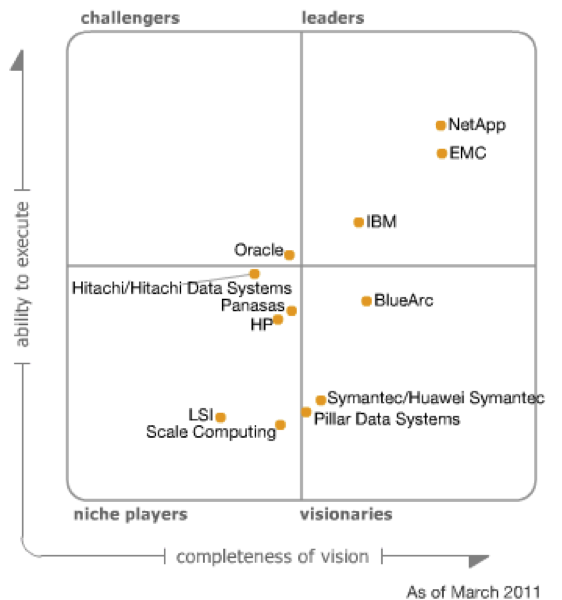
\includegraphics[, keepaspectratio = true]{media/magicquader_nas.png}
\mycaption{figure}{\label{abb:MagicQuaderNAS} Gartner Magic Quader März 2011}
\end{center}

\paragraph*{Modulare Disk Array Speicher}
Gartner hat die Anbieter von Modularen Disk Array im mittleren und oberen Bereich auf Ihre Marktchancen untersucht und hat dieses in Marktführer, Herausforderer, Visionär und Nichen Anbieter eingeteilt. Es wurden nur Anbieter berücksichtig die Modularen Disk Array Lösungen ab einen Preis von 25'000\$ anbieten und in den Märkten Nord Amerika, EMEA oder Japan und Asien Pazifik vertreten sind.

Als Marktführer wurden Anbieter, welche einen bedeutenden Marktanteil haben, ausreichend Marketing- und Verkaufs-Kapazitäten haben und Technologisch führend und Innovativ sind.

Als Herausforderer gelten Anbieter mit einen starken Produkt die einen glaubhaft Marktanteil und Ressourcen diesen ausbauen zu können. Die Anbieter sind jedoch zu wenig Visionär um sich als Marktführer zu qualifizieren.

Als Visionäre gelten Anbieter die eine einzigartige Innovative Produkte haben, die Operationelle oder Finanzielle wichtige End-Benuzter Probleme adressieren, aber noch nicht bewiesen haben einen substantiellen Marktanteil aufzubauen.

Als Nischen Anbieter gelten als Anbieter welche Spezielle Produkte haben die auf einen spezifischen Markt oder Segment ausgerichtet sind.

Wie aus der \refabb{abb:MagicQuaderModularDiskarrays} zu entnehmen ist Stuft Gartner EMC, NetApp, HP, Dell und Hitachi Data System zu den Marktführer ein. Oracle und Fujitsu sieht Gartner als Herausforderer an und XIO wird als visionare bezeichnet.
 
\begin{center}
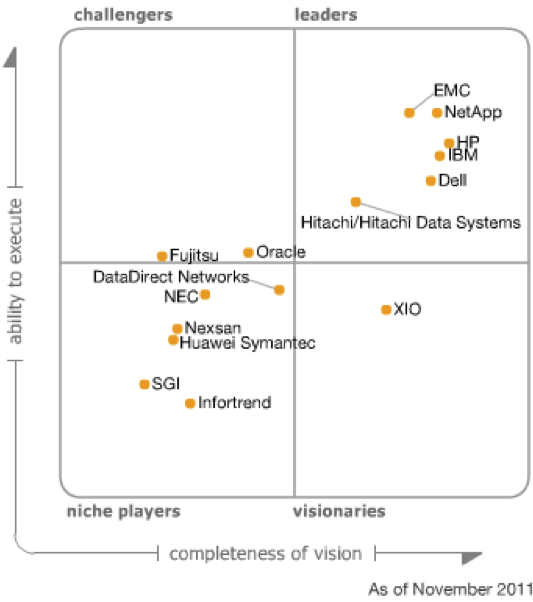
\includegraphics[, keepaspectratio = true]{media/magicquader_modulardiskarrays.png}
\mycaption{figure}{\label{abb:MagicQuaderModularDiskarrays} Gartner Magic Quader Modular Disk ArrayMärz 2011}
\end{center}


\paragraph*{Distributed Filesystem Cluster Speicherlösungen}
Zu den bekannten Vertreter der Distributed Filesystem gehören Hadoop HDFS, Gluster, Lustre, alle drei haben gemeinsam dass es sich bei den Lösungen um Open Source Software handelt.

Hadoop basiert auf dem Designs Konzept von Google Filesystem und Google Mapreduce. The Guardian hat Apache Hadoop 2011 als Erfinder von Jahr ausgezeichnet. InfoWorld hat Hadoop für den InfoWorld 2012 Technology Award ausgewählt und für Gartner zählt Hadoop zu den top 10 Technologie Trends welche Einfluss auf die Informatik Infrastruktur nehmen. 
Zu dem Prominenten Unternehmen die Hadoop einsetzen und mitentwickeln zählen Yahoo und Facebook. Neben den beiden genannten gibt es weiter viele namhafte Unternehmen wie IBM, AOL, Twitter und weiter die Hadoop einsetzen. \cite{Guardian}\cite{Wayner2012}\cite{Casonato2012}\cite{Hadoop2012}

GlusterFS wurde von der Firma Gluster Inc. als Opensource Projekt entwickelt. Im Jahr 2011 wurde GlusterInc von der Firma Red Hat Inc. übernommen um Lösungen für den Big Data Bereich anbieten zu können. Red Hat wurde mit der Übernahme von Gluster Inc zum Haupt unterstützer von GlusterFS.

\paragraph*{Online Speicher}
Einer der ersten grossen und wohl der bekannteste Online Speicher Anbieter zählt Amazone mit Ihren S3 Produkt. Amazone veröffentlich zwar keine Finaz Daten über Ihre Cloud Produkte, jedoch haben Sie Daten über das Wachstum der Anzahl gespeicherten Objekten veröffentlicht. So Speicherten hatten Sie im Jahr 2006 ca. 2.9 Milliarden Objekte gespeichert, im Jahr 2010 wahren es bereits 269 Milliarden Objekte dieses Ergebnis konnten Sie jedoch auf das Jahr 2011 mit 762 Milliarden Objekten mehr als verdoppeln. \cite{Barr2012}

\begin{center}
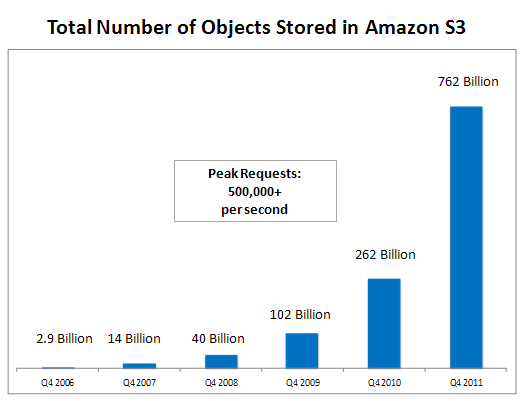
\includegraphics[, keepaspectratio = true]{media/s3_growth_2011_3.png}
\mycaption{figure}{\label{abb:AnzahlObjekteAmazonS3} 
\cite{Barr2012}Anzahl gespeicherte Objekte in Amazon S3 \cite{Barr2012}}
\end{center}

Neben Amazon zahlt RackSpace zu den führenden Cloud Anbietern, wie Amazon bietet auch RackSpace den Online Speicher an. Ihr Online Speicher wird unter der Produkt Bezeichnung Cloud File verkauft. Hinter Cloud File steckt eine von Ihnen selbst entwickeltes Speicher genannt OpenStack Object Storage Code Name Swift. RackSpace hat an OpenStack Object Storage ein Jahr lang entwickelt und diese wie Ihre anderen Cloud Eigenentwicklung als Quelloffenes Projekt unter OpenStack veröffentlicht. Zu OpenStack tragen neben Rackspace weitere nahmhafte Unternehmen wie Dell, HP, Citrix, AMD, NetApp, Suse, AT&T, NASA und weitere Unternehmen bei.
RackSpace setzt dazu von Ihnen selbst entwickelte OpenStack Object Storage als Online Speicher ein. \cite{OpenStack}

In der Schweiz ist die Entwicklung von Cloud Storage noch nicht so weit an geschritten wie in Vereinigten Staaten, zu den wenigen Anbieter gehört Swisscom.


\section{Trend}
Für Gartner zählen Modular Disk Array Speicher und NAS zu den etablierten Speicherlösungen. Online Speicher (Cloud Storage) sieht Sie als Speicherlösungen welche sie    
Gartner untersucht jährlich die Hypes und o

weshalb wiso warum

wenig anbieter welche grosse datenanbieter 

statistic massendaten